\documentclass[final]{IEEEtran}
\usepackage{cite}
\usepackage{amsmath,amssymb,amsfonts}
\usepackage{algorithmic}
\usepackage{graphicx}
\usepackage{textcomp}
\usepackage{xcolor}
\usepackage{datetime}
\usepackage{seqsplit}

\graphicspath{{./images/}}
\def\BibTeX{{\rm B\kern-.05em{\sc i\kern-.025em b}\kern-.08em
    T\kern-.1667em\lower.7ex\hbox{E}\kern-.125emX}}
\begin{document}

\title{ Scam Booter\\\vspace*{10pt} \LARGE CPEN442 \\\vspace*{10pt} \large November 9}
\author{\textbf{Zoy Huang (20026150), Ryan Koon (11062149), and Wendy Zhou (41378150)}\\
Department of Electrical and Computer Engineering\\
University of British Columbia\\
Vancouver, Canada

%\\\vspace*{10pt}
%emailA.com, emailB.com, emailC.com
}
\maketitle

% The abstract should summarize the problem addressed, methodology, results, conclusions, and contributions.
\begin{abstract}
Technical support scams have been a growing issue as more financial losses have been reported year after year. Software companies like Microsoft and Google have been improving their software security and processes to block malicious websites as well as working with law enforcement to tackle the issue. There is no perfect solution and user education is the most effective provided that the information reaches those that will benefit from it. Therefore, to provide an extra line of defense, we created ScamBooter to detect remote connections and analyse interactions with administrative applications on Windows. If malicious behaviour is detected, we attempt to terminate the user’s connection with the scammer and provide details about the scam so that the user is better equipped to avoid falling for a technical support scam in the future. This further promotes user education of the issue.

We built and tested our solution based on scenarios and statistics provided by a large-scale analysis conducted on technical support scams. Due the rapidly changing environment of cybercrime, we can only deem our solution as a part of a multi layer defense system. Ideally, our heuristics in detecting a scam and the implementation recover from from a scam would be used to enhance an existing security software solution or built into an operating system. Alternatively, operating systems can restrict access to adminstrative applications not often used by general users. In addition, they should provide descriptions in plain English on what the applications can and cannot do before allowing the user to enable them. However, we cannot expect a user to read the description and make the expected choices under the direction of a scammer. Therefore, automated solutions still has it place in protecting users.
\end{abstract}


\section{Introduction} % 10%
%================================================================================================================
%The section should provide the following
%
%1. Explain clearly the problem addressed by your project.
%2. Explain why this is an important problem.
%3. Summarize the designed system
%4. Summarize related work.
%5. Summarize the methodology that you have followed for evaluating your design.
%6. *Summarize evaluation results you obtained .
%7. *Summarize the conclusions your drew from the results.
%8. List contributions of your project.
%
% *Only for the final Report
%================================================================================================================

\subsection{What is the problem that we addressed?}
%===============================
We addressed the issue of social engineering from technical support scams, which has caused an increasing trend of reported financial losses \cite{b1}. We proposed a solution that protects users with little knowledge about Windows' administrative tools. The asset at risk is the victim's bank account. The vulnerability is the victims lack of knowledge about Administrative tools on Windows. The threats are people pretending to be legitimate technicians and deceiving users about the state of their computer.

\subsection{Why is this problem important?}
%===============================
According to Microsoft, there were 153,000 technical support scam reports worldwide in 2017, a 24\% growth from the previous year \cite[Fig 1]{b3}. In the same year, the Internet Crime Complaint Center (IC3) received approximately 11,000 technical support complaints that totals to a loss of almost \$15 million. That was an “86\% increase in losses from 2016” \cite{b1}. In a recent study (September 2018) released by Microsoft, financial losses have become more consistent worldwide as some countries have experienced less losses while others have experienced an increase in losses \cite[p.12]{b7}. Not only is financial loss an issue but 52\% of surveyed users spent time finding out what was wrong with their computer and "three-in-four consumers who continued with a scam experienced moderate to severe stress" \cite[Fig 3]{b7}.

\begin{figure}[htbp]
\centerline{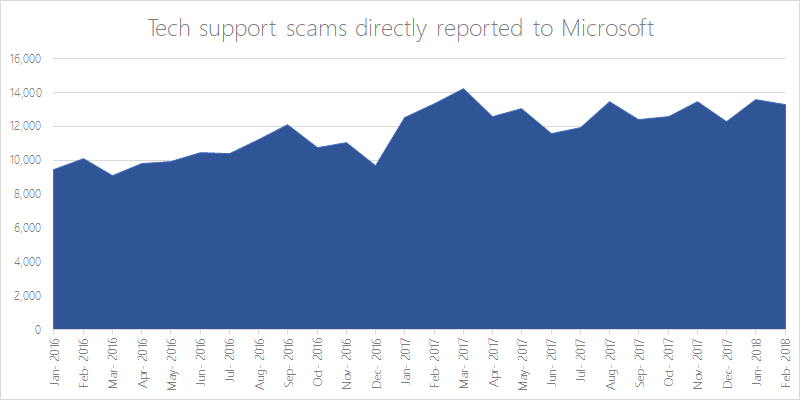
\includegraphics[keepaspectratio=true, scale = 0.32]{image1.png}}
\caption{Number of tech support scams reported to Microsoft}
\label{fig2}
\end{figure}

A study \cite{b2} conducted in 2014 discovered 1,688,412 unique visitors to scam sites and estimated a loss of at least \$9.7 million. With this trend, it appears that technical support scams are not going away even with efforts to stop them \cite[p. 8]{b2}.

\begin{figure}[htbp]
\centerline{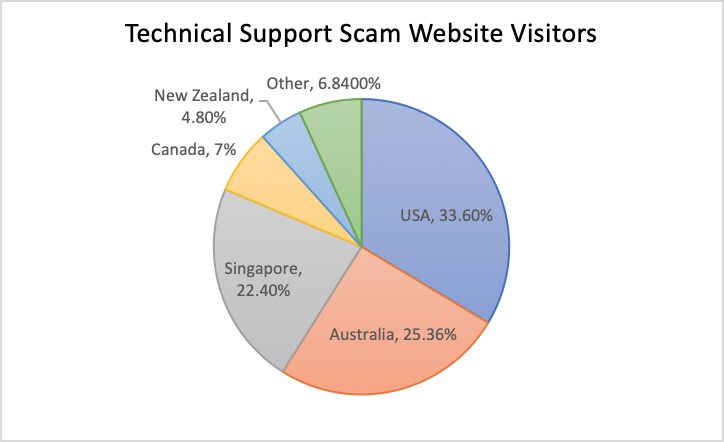
\includegraphics[keepaspectratio=true, scale = 0.30]{image0.png}}
\caption{Tech support scam website visitors by country}
\label{fig1}
\end{figure}

\begin{figure}[htbp]
\centerline{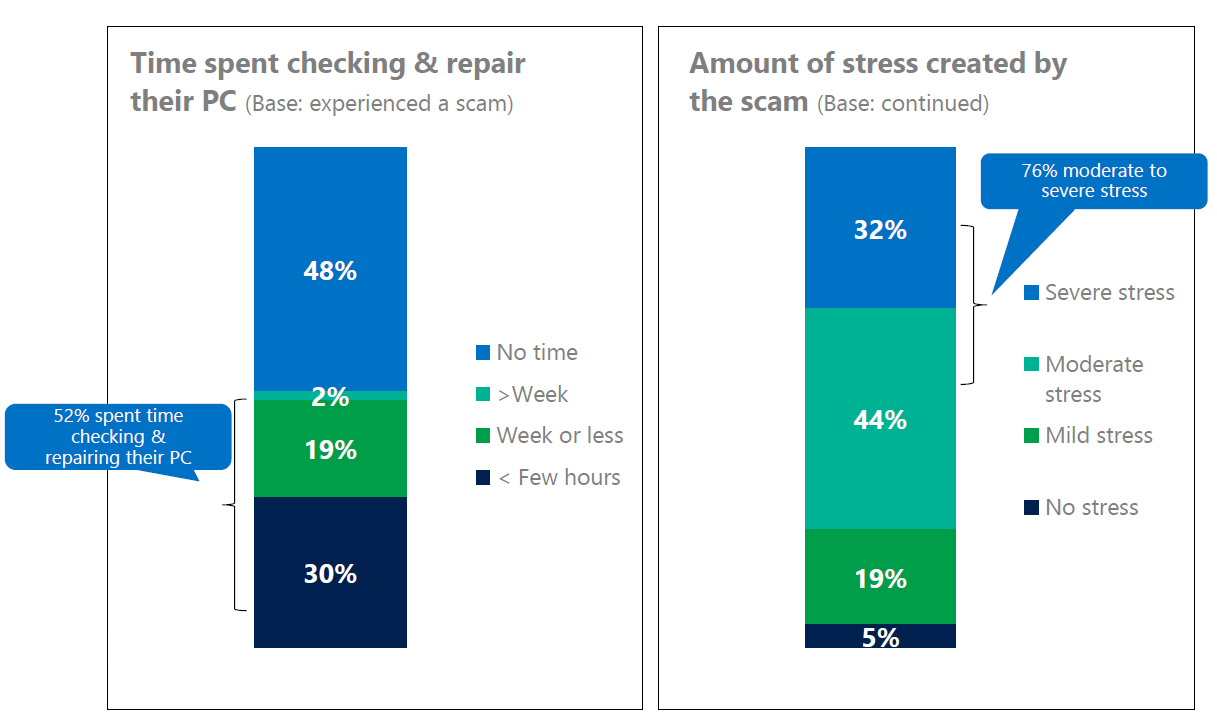
\includegraphics[keepaspectratio=true, scale = 0.28]{timeandstress.png}}
\caption{Time spent fixing computer and stress levels}
\label{fig3}
\end{figure}

\subsection{Summary of the Designed System}
%===============================
Social engineering attacks thrive on human error based on an inadequate knowledge of the system being used. A novice user does not have the knowledge to recognize fallacies provided by the technical support scammer, nor do they have working knowledge of Windows tools used to manipulate them.

However, notably, scammers follow similar sequences of events and use similar techniques to convince their victims. The most common techniques are shown in \cite[Fig 4]{b2}.
\begin{figure}[htbp]
\centerline{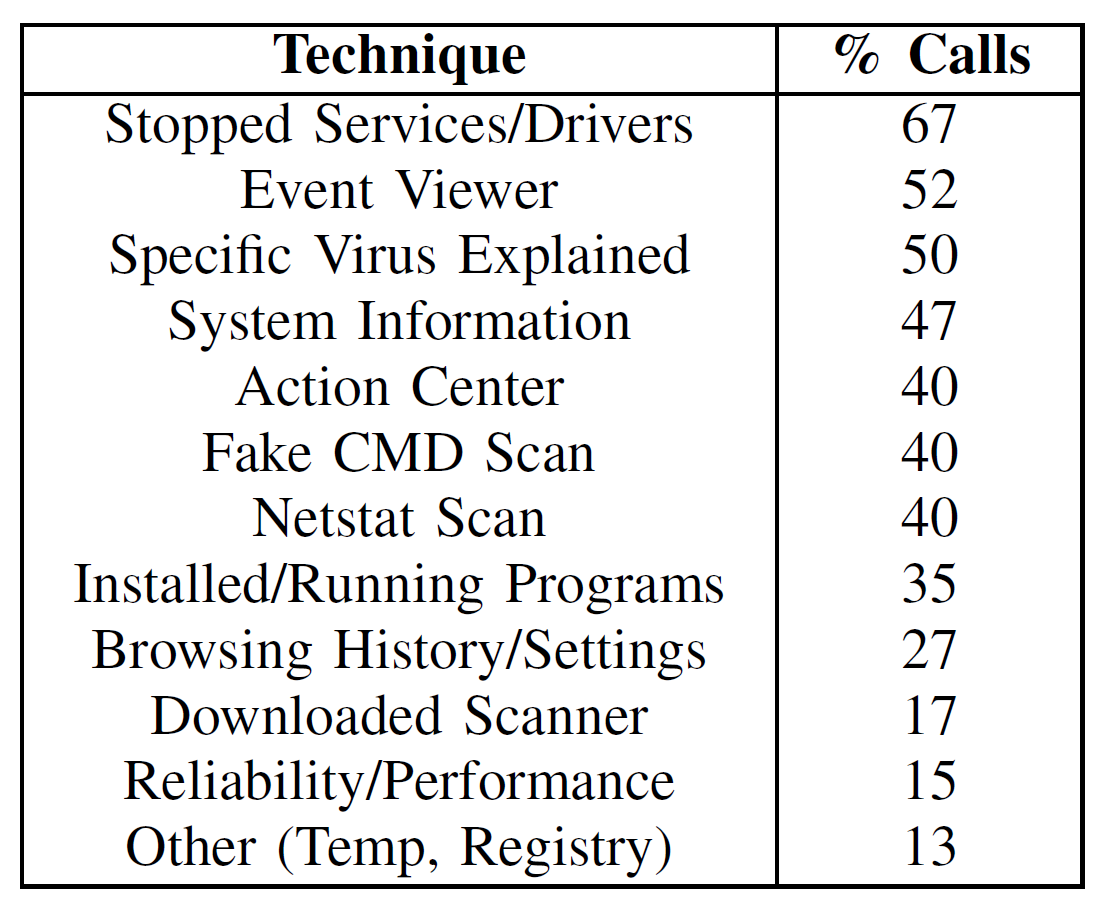
\includegraphics[keepaspectratio=true, scale = 0.20]{image3.png}}
\caption{Techniques used by support scammers in order to convince their victims of a malware infection}
\label{fig4}
\end{figure}

We defined these events and techniques as ``suspicious behavior''. For example, the use of the administrative tool, ``Event Viewer'', qualifies as suspicious behavior. Our solution, called ScamBooter, protects users that lack knowledge about the tools and techniques used in technical support scams by detecting these events on their behalf.

We addressed the problem by using the Windows API to build a Windows application that detects the suspicious behaviors. If a scam is detected, the application forcefully terminates commonly used remote access applications in this type of scam and informs the user of the event. We also prevented the application from being terminated by creating a Windows service that manages the lifecycle of the application. In certain scenarios, we analysed keystrokes to more accurately determine whether a scam is in progress. To ensure our application is compatible with consumer security solutions, we tested our programs in environments installed with security software from major security software vendors such as Norton Security and Sophos.

As an overarching goal, we aimed to protect users from malicious remote access to their computer and to educate them in a timely manner on technical scams. This was also an exploration into how we can provide security via behavioural analysis without severely impacting the user experience of Windows.

\subsection{Summary of Related Works}
%===============================

ROBOVIC, short for Robotic Victim, was a tool created in a study that collected data about technical support scams. It crawled the web to find websites, its visitors, and phone numbers used for these kinds of scams \cite[Fig 2]{b2}. The investigators concluded that “the vast majority of AV users are likely not going to be protected against technical support scams”  \cite[p.7]{b2}. On average, 64\% of 1624 malicious TLDs (Top Level Domains) were only detected by 3.25 AV engines out of 68 engines \cite[p.7]{b2}. Phone applications on Android detected “less than 1\% of the 1,581 scammer-operated phone numbers” \cite[p.8]{b2}. On average it took 44 days for a phone number to be reported as a part of a scam. Even worse, some mobile applications associated scam numbers with positive reviews and legitimate businesses such as Dell and McAfee. Microsoft has been making a wide range of improvements by “enhancing antivirus, email, URL blocking, and browser security solutions”. TeamViewer has been displaying prompts to warn users about technical support scams. In terms of user education, attempts such as public service announcements have been made. However, they were ineffective being on specific sites that were not known by the general population  \cite[p.13]{b2}. Having their customers as being the major target for technical support scams, Microsoft have been dedicating more resources into the issue and working with law enforcement to track down the scammers.


%NOTE: Should probably get some academic sources for this section, and rewrite it. +++++

\subsection{Summary of the Methodology}
%===============================
To test our detection rate, we compiled a suite of known remote connection programs and known windows administrative tools.
For testing key logging We constructed a test suite that contains various forms of malicious strings and harmless strings.
We assessed the effectiveness of our solution based on the number of detected processes or strings in the test suite.

%\subsection{Summary of Evaluation Results}
%===============================
% %Only for the final Report

%\subsection{Summary of our Conclusion}
%===============================
% %Only for the final Report

% Existing solutions include informing the user through online information, blacklisting scammers' numbers and domain names, and antivirus solutions. Blacklisting scammer websites and phone numbers is not an effective method since the scammers can always register new domain names, create new websites, and use other phone numbers. Our solution focused on detecting a potential scam on the user's system and immediately brings them back to safety. It protects users who are experiencing potential phone scams and does not rely on numbers and IP addresses of scammers. The goal of our system was not only prevention but also detection and recovery. This can be considered a layer of defense inside a “fortress”, which helps protect inexperienced users.

\subsection{List of Contributions}
%===============================


\section{Related Work} % 5%
%================================================================================================================
% This section should explain what others, particularly as reported in academic literature, have done designing systems similar to the one designed by your team.
%================================================================================================================
Besides the large scale analysis conducted by researchers from Stony Brook University, there has not been any new academic studies in this area \cite{b2}. However, there has been widespread media coverage of call centre raids \cite{b6}. In fact, the increased in usage of pop-up ad-blockers potentially reduced the likelihood  of preventing exposure to scam websites, one of the entryways into a technical support scam \cite{b7}. Microsoft's Digital Crimes Unit has continued to conduct investigations, collect evidence, and work with law enforcement to combat technical support scams. This year, google has started restricting ads that claim to provide technical support services by starting a verification program to ensure that only legitimate third-party technical support providers are using their advertising platform \cite{b8}. Scammers are developing new ways trick people in making a payment and certainly more effort has been put into blocking websites and ads. However, analysing user behaviour as the last line of defense is not seen in products for the mass market. This could be due to resource limitations of most consumer computers to be able to provide detailed and accurate analysis as well as privacy concerns. The best solution is providing user education on this issue and there are plenty resources on such scams and many others \cite{b10}. The problem is being able to reach out to those that will benefit from the information.




\section{Adversary Model} % 9%
%================================================================================================================
% Describe the adversary model that your design is intended to resist.
%================================================================================================================
Although there are various techniques that are used by technical support scammers, we developed a generalized model by analyzing the patterns of technical support scams. This model facilitated our understanding of the problem and helped us to design our system.
\subsection{Objectives}
The objective of the adversaries is to convince the victim that their computer is infected by a virus. After gaining the trust of the victim, the adversaries make the victim to pay them for fixing non-existent problems. The adversaries are scammers who want to make profits by deceiving inexperienced Windows users.
\subsection{Initial capabilities}
The adversaries can call users, claiming to be from well-known companies. The adversaries can also set up malicious websites or advertisements that tell the user to call technical support numbers. 
\subsection{Capabilities during the attack}
The adversaries ask a user to download remote access software and gain access to their computer. They can open administrative tools to show system "errors", which are logs of normal operation. They can install malwares on the user's machine, causing the machine crash.

\section{System Design} % 20%
%================================================================================================================
% 1. This section should explain the most interesting parts of your design.
% 2. Provide rationale for the design decisions.
% 3. Explain which principles of designing secure systems have been employed by your design.
%===============================================================================================================

\subsection{Detecting a remote connection}
%===============================
Detecting an active remote desktop connection is not as trivial as checking a flag. For Windows, that is only possible if the application is using the Microsoft Remote Desktop Protocol, which operates on specific ports. However, the remote desktop applications used by technical support scammers typically establish connections on port 80 and 443, the standard ports used by web clients to communicate with a machine. Also, these ports are only used to establish a connection, the resulting port is not the same for each session as it is assigned by the machine serving the desktop. Other non-standard ports are used by remote desktop applications, but they differ between software, they may not be documented, or the ports they use will change depending on network conditions. Such a moving target will result in a high rate of false-positives. Instead of analysing network traffic, our application analyses raw input data using the Windows Desktop API \cite {b4}. Every time a mouse click occurs, regardless of the application in focus, our application will check whether a handler to the device is provided in the raw input header. If so, it is a local device that is attached to the computer. If no handler is provided, it is an input made from an active remote connection to the computer. Using this method, we can distinguish between clicks from a locally connected mouse and clicks from a remote desktop application.

\subsection{Detect the use of administrative tools}
%===============================
As illustrated in \cite[Fig 2]{b2}., scammers use specific Windows programs during an attack. 67\% of scammers start services.exe to show users a list of stopped services. 52\% calls to Event Viewer, 40\% calls to Netstat and 40\% calls to Command Prompt. Since the calls to these tools are closely related to a scam in progress, we decided to monitoring the use of these administrative tools. To implement this, our application registers a WMI (Windows Management Instrumentation) event handler to receive notifications of the start of a process \cite{b9}. We check if the launched process includes services.exe, eventvmr.exe, mmc.exe, cmd.exe or netstat.exe. We assume users who have extensive knowledge of windows administrative programs are not susceptible to technical support scams. The use of particular administrative programs for a typical user would be an abnormal. 

\subsection{Analysing keystrokes}
%===============================
To improve the accuracy of detecting a scam in progress, we log keystrokes when the Windows Command Prompt is in focus. Scammers frequently execute certain commands to trick the user into believing that there is malware on their computer. 40\% of scammers employ a “Fake CMD scan” by running a command to list the tree of files, folders, and subfolders at a certain path \cite[p.7]{b2}. Our application will capture keystrokes that occur while the command prompt is outputting information. We will look for common words and phrases typed in such as “Virus detected”. We employ this strategy because users are often tricked into believing that the system produced the output not knowing that user inputs are displayed after a command is done executing. To capture keystrokes we use a global hook open source library that will allow our application to learn about keystrokes regardless of the application in focus \cite {b5}.

\subsection{Terminating remote access applications}
%===============================
Stopping all network traffic would be a fail-safe strategy to terminate the connection between the user and the scammer. However, this will affect all other applications that require network connectivity which arguably, makes our application appear to be malware. To prevent such degradation to the user experience, we terminate common remote desktop applications used by technical support scammers instead \cite[Fig 4]{b2}. Our application runs with elevated privileges to allow us to terminate remote access applications with elevated privileges and to counter process renaming done via a file rename. We access the file metadata to determine the original name of the application rather than relying solely on the process name.

\begin{figure}[htbp]
\centerline{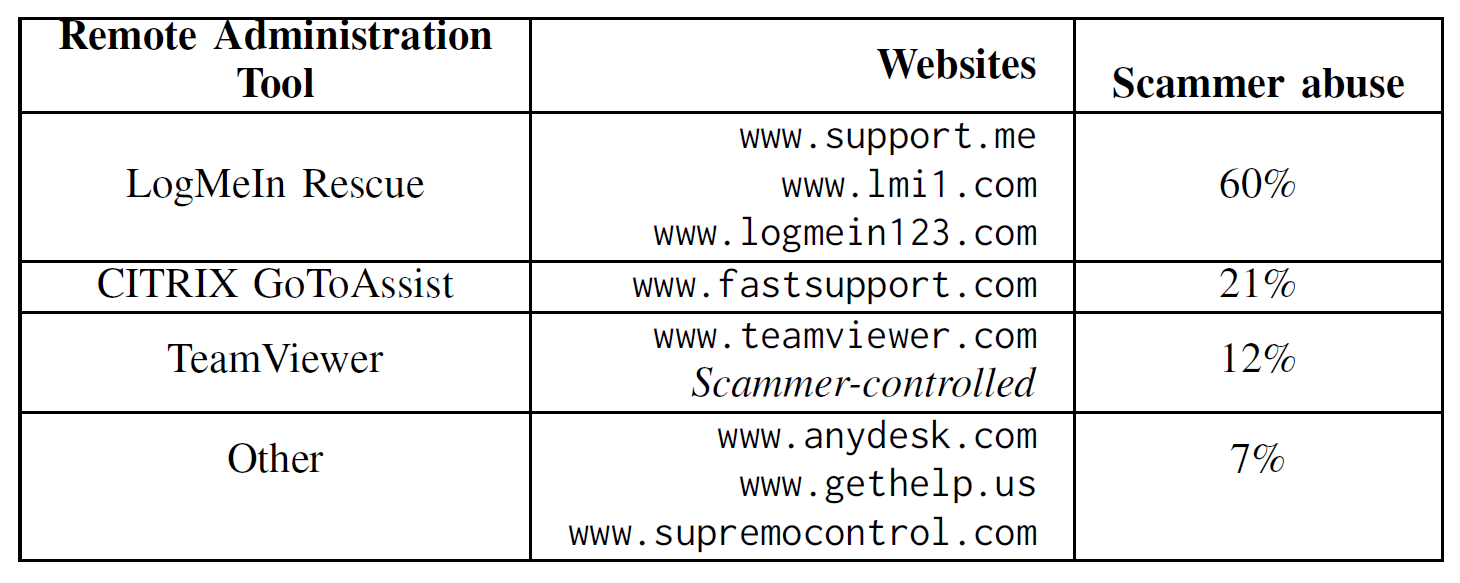
\includegraphics[keepaspectratio=true, scale = 0.22]{RemoteTools.png}}
\caption{Remote access tools used by technical support scammers.}
\label{fig 4}
\end{figure}

\subsection{Self restarting}
%===============================

\subsection{Principles of design}
%===============================
We applied the following principles to our system design.
\begin{itemize}
  \item\textbf{ Psychological Acceptability.} It is easy for users to install and start our system. Our system shows messages that inform users about potential scam activities. 
  \item\textbf{ Defense in Depth.} By implementing a Windows service program that launches on startup and restarts our application program, we prevented our application from being terminated by scammers. This added a layer to protect the system. 
\end{itemize}
%===============================

\section{System Prototype} % 15%
%================================================================================================================
% Explain the details of the prototype of your approach. This is the prototype that is used for evaluating your approach.
%================================================================================================================
Our prototype consists of (1) a Windows application that detects suspicious activities and (2) a Windows service that manages the lifecycle of the application. We developed two programs using C\# and .NET framework. 

\subsection{Windows application}
The application is responsible for detecting and terminating potential technical scam activities. It monitors the launched processes including event viewer and command prompt and detects remote connections using raw mouse input. Based on these two factors, the application predicts if there is a possible scam activity and notifies users.\\
In extreme cases, our application terminates remote connections by disconnecting user computer from the Internet for a short period of time. It displays a message to explain the reason for disabling the Internet and direct users to to reputable page about tech scams.

\subsection{Windows service}
The role of the service is to prevent the application from being terminated. It checks the list of running processes at a set interval and restarts ScamBooter if the application is not running.

\section{Evaluation} % 26%
%================================================================================================================
% This section should provide details of the evaluation, using the following sub-subsections.
%
% 1. (A. Evaluation Methodology) (12%) This subsection should explain how the system was evaluated. Focus on the most important for the reader elements of your evaluation.
% 2. *(B. Results of the evaluation) (7%) This section should describe the results of the evaluation. Remember to keep the description of the evaluation and the description of the results in separate sub-sections.
% 3. *(C. Discussion of the evaluation results) (7%) This section should discuss what the results of the evaluation mean.

%The above enumerated items should be discussed in separate subsections of Methodology section. Their titles are suggested in the parenthesis.
% *Only for the final Report
%================================================================================================================



\subsection{Evaluation Methodology}
%===============================

We determined a list of success criteria for our program: Fraud rate, insult rate, Psychological acceptability.

To assess fraud rate of programs we run the entire list of windows administrative tools and popular remote connection software (seem in Fig. 4) against our program. The target fraud rate is 0 where our program detects each item on the list.

Based on our threat model, users who can trigger our detection system on their own have enough technical knowledge to be safe from technical support scams. Therefore, the insult rate for programs will not be a significant metric in our evaluation. 

However, our program also performs key logging to check it for intrusion.
To assess the fraud rate of the key logger, we will test it against strings of input known to be part of a scam.
To assess the insult rate for our key logger, we will test it against harmless common text found in online databases such as books, blogs, as well as random generated text.

A limitation of our design is that our detection works based on the signatures of programs. The program can only correctly identify software that is known to be used in combination for software scams. Therefore, we will not evaluate unknown programs, and expect signature updates to patch breaches using unknown programs.

One other important metric is Psychological acceptability: Users should not be aware of our program running in the background.
The assess this criteria, we ran the program, and check these places for traces of the program running: Task Bar, application switch window, timeline, action center, and program icons. Eliminating traces from these menus render our program invisible, and only seem as a background process.


%\subsection{Results of the Evaluation} % 10%
%===============================
%%Only for the final Report

%\subsection{Discussion of the Evaluation Results} % 10%
%===============================
%%Only for the final Report







%\section{Discussion} % 10%
%================================================================================================================
% Discuss pros and cons of your design, as well as limitations and advantages of it. This discussion should integrate the related work, the motivation for the design, the adversary model, the ideas of the design, and the results of the evaluation. This section should be about one page. 
%Only for the final Report
%================================================================================================================

%\section{Conclusion} % 5%
%================================================================================================================
% This section should summarize the report in 1-2 paragraphs. Although a conclusion may review the main points of the report, do not replicate the abstract as the conclusion. A conclusion might elaborate on the importance of the work or suggest applications and extensions.
% Only for the final Report
%================================================================================================================


\begin{thebibliography}{00}
\bibitem{b1} Federal Bureau of Investigation, ``TECH SUPPORT FRAUD'',  https://www.ic3.gov/media/2018/180328, Mar. 28, 2018 [Oct. 6 2018]
\bibitem{b2} N. Miramirkhani, O. Starov, and N. Nikiforakis, “Dial One for Scam: A Large-Scale Analysis of Technical Support Scams,” in Proceedings 2017 Network and Distributed System Security Symposium, 2017
\bibitem{b3}E. Wahlstrom, “Teaming up in the war on tech support scams,” Windows Server Blog, 06-Jun-2018. [Online]. Available: https://cloudblogs.microsoft.com/microsoftsecure/2018/04/20/teaming-up-in-the-war-on-tech-support-scams/. [Accessed: 06-Oct-2018].
\bibitem{b4}"C\# Get Mouse handle (GetRawInputDeviceInfo)", Stack Overflow, 2018. [Online]. Available: https://stackoverflow.com/questions/14584280/c-sharp-get-mouse-handle-getrawinputdeviceinfo. [Accessed: 09- Nov- 2018]
\bibitem{b5}"rvknth043/Global-Low-Level-Key-Board-And-Mouse-Hook", GitHub, 2018. [Online]. Available: https://github.com/rvknth043/Global-Low-Level-Key-Board-And-Mouse-Hook. [Accessed: 09- Nov- 2018]
\bibitem{b6} S. Chabba, “Indian Fake Call Centers Scam Americans Of Millions Of Dollars, 70 Suspects Arrested,” International Business Times, 06-Oct-2016. [Online]. Available: https://www.ibtimes.com/indian-fake-call-centers-scam-americans-millions-dollars-70-suspects-arrested-2427340. [Accessed: 10-Nov-2018]
\bibitem{b7} “Global Tech Support Scam Research - Global Summary, September 2018.” [Online]. Available: https://news.microsoft.com/uploads/prod/sites/358/2018/10/Global-Results-Tech-Support-Scam-Research-2018.pdf.
\bibitem{b8} D. Graff, “Restricting ads in third-party tech support services,” Google, 31-Aug-2018. [Online]. Available: https://www.blog.google/products/ads/restricting-ads-third-party-tech-support-services. [Accessed: 10-Nov-2018].
\bibitem{b9}"Receiving a WMI Event", Microsoft, 2018. [Online]. Available: https://docs.microsoft.com/en-us/windows/desktop/WmiSdk/receiving-a-wmi-event\#event-consumers. [Accessed: 09- Nov- 2018]
\bibitem{b10}“Protect yourself from tech support scams,” Microsoft Support. [Online]. Available: https://support.microsoft.com/en-ca/help/4013405/windows-protect-from-tech-support-scams. [Accessed: 10-Nov-2018]
\bibliographystyle{IEEEtran}
\end{thebibliography}

\end{document}
